
\section{Utils} 

Im Utils namespace sollen sollen sich folgende Hilfsfunktionen zur Zeit/Datumsumrechnung befinden.

\begin{itemize}
\item Umrechnung in einen Dauer-String Bsp.: ,,4 hours 2 minutes 0 seconds''

\begin{verbatim}
Glib::ustring seconds_to_duration(unsigned long);
\end{verbatim}

\item Umrechnung in einen Timestamp, Bsp: ,,2011-04-02''
\begin{verbatim}
Glib::ustring seconds_to_timestamp(const long);
\end{verbatim}

\item Umwandlung eines Integer Wertes in einen String
\begin{verbatim}
std::string int_to_string(int num); \end{itemize}
\end{verbatim}

\end{itemize}


Diese grundlegenden Funktionen sollen ausgelagert werden damit sie von mehreren Klassen verwendet werden können und um Redundanzen im 
Code zu vermeiden.


\section{Config}
%Beschreibung der load/save Funktionalität siehe model_save_load.txt
\subsection{Hauptklassen}

%----------------------------------------------------------------------------------------------

\subsubsection{Path}
Die \emph{Init::Path} Klasse soll für die Initialisierung und das Management der Freya Config Pfade zuständig sein.
Bei der Initialisierung soll überprüft werden ob das Konfigurationsverzeichnis vorhanden ist, wenn nicht wird ein Neues
angelegt und anschließend wird eine default config.xml geschrieben. Eine default config ist im Quellcode als 
globaler konstanter String einkompiliert. (Config::defaultcfg.inl)
\\
\\
Schlägt das Erstellen der Konfigurationsdatei fehl, so soll versucht werden eine entsprechende Fehlermeldung in die Log Datei zu schreiben 
falls diese zuvor erfolgreich angelegt wurde. Zusätzlich sollen DEBUG Ausgaben auf dem Bildschirm angezeigt werden wenn das Programm
über ein Terminal gestartet wird.

    %----------------------------------------------------------------------------------------------

\subsubsection{Model und Konfigurationsdatei}

Die Freya Konfigurationsdatei soll im simplen XML Format realisiert werden, XML wird gewählt um das Parsen zu vereinfachen und um
ein standardisiertes Format nach außen bereitzustellen. 
\\
Die Konfigurations- und Logdatei soll nach XDG Standard \verb+($XDG_CONFIG_HOME)+ unter \verb+$HOME/.config/freya/<config.xml,log.txt>+ gespeichert werden.
\begin{itemize}
\item \begin{verbatim}
	http://standards.freedesktop.org/basedir-spec/basedir-spec-latest.html#variables
\end{verbatim}
\end{itemize}

Die Optionen in der Konfigurationsdatei sind baumartig nach ,,Domainprinzip'' aufgebaut. Die Konfigurationsdatei unter \ref{c_config}
zeigt exemplarisch einen möglichen Aufbau.


\begin{figure}[h!]
\lstinputlisting[language=XML]{config.xml}
\caption{Die Konfigurationsdatei im XML Format}
\label{c_config}
\end{figure}

Die \emph{Config::Model} Klasse gehört nach dem MVC Paradigma zur Model Schicht. Diese Klasse soll die nötigen Daten (Konfigurationsdatei)
die zum Betrieb von Freya nötig sind im Speicher vorhalten und Methoden zum Lesen und Speichern der Konfigurationsdatei auf die Festplatte 
bereit stellen.

Zum Parsen der XML Datei soll hier die C Programmbibliothek libxml2 verwendet werden. Diese Library wurde gewählt, weil sie alle benötigten Funktionen enthält, nach dem ANSI-C Standard implementiert ist
und bereits seit über einem Jahrzehnt Quasi-Standard im C Umfeld ist.

Zu verwendende Libraries:
\begin{itemize}
    \item \url{http://xmlsoft.org/}
    \item \url{http://en.wikipedia.org/wiki/Libxml2}
\end{itemize}

%Hier das Sequenzdiagramm vom Model


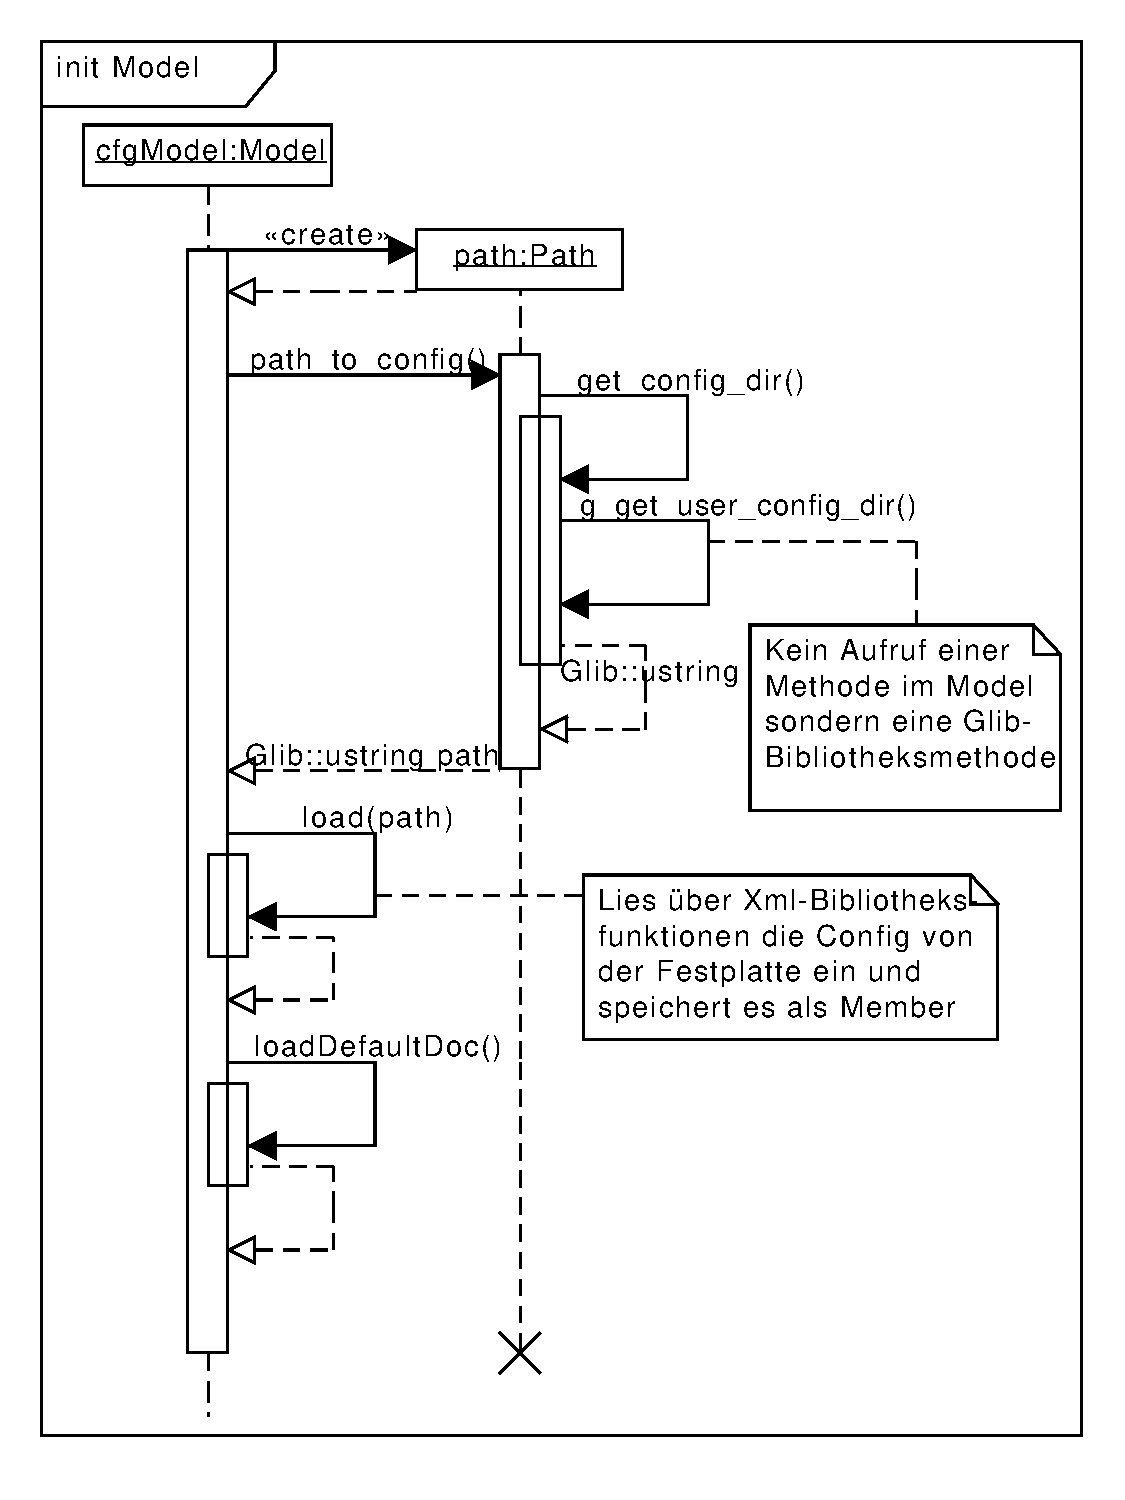
\includegraphics[scale=0.6]{init.pdf}
%\caption{Initialisierung des Models}
\label{c_modelinit}

\subsection{Initialisierung des Models}

 
Über die Init::Path Klasse holt sich das Model bei seiner Instanziierung über die path\_to\_config() Methode
den Pfad zur Konfigurationsdatei, parst diese sowie die default Config und 
initialisiert zwei XML Document Pointer die auf ein DOM Objekt, welches einen Dokumentenbaum enthält, zeigen.
Hierzu werden die load(pathtofile) und die loadDefaulDoc() Methoden der Config::Model Klasse verwendet.
\\   

Anschließend kann man über diese DOM Objekte traversieren und Werte der Konfigurationsdatei lesen oder setzten.
Die default config wurde implementiert um fehlerhaften Werten oder einer kaputten Konfiguration vorzubeugen. Ist ein benötigter Wert
nicht in der User config vorhanden oder ist diese beschädigt so wird auf die default config zugegriffen.
Bei Beendigung des Models wird das aktuelle Objekt als XML Konfigurationsdatei auf die Festplatte geschrieben.
Wie andere Objekte auch, nutzt das Model die Log-Klasse um zu Informationen und Fehler zu protokollieren.


\subsection{Prinzipieller Ablauf der load() Methode}

Beim Instanzieren ruft das Model seine load() Methode auf mit dem aktuellem Pfad auf
in dieser wird als Erstes die libxml2 Methode xmlParseFile(pathtofile) aufgerufen. Diese bekommt den
Pfad zur Konfigurationsdatei übergeben und versucht über den übergebenen Pfad zu das File zu laden.
An den ,,xmlNodePtr curNode'' Pointer wird der Rückgabewert der xmlParseFile() Methode zurückgegeben,
wenn die Operation erfolgareich war, ansonsten \emph{NULL}.

Anschließend wird das geladene Dokument geprüft, ist dieses \emph{NULL} so wird eine entsprechende Fehlermeldung
über den Logwriter in die Logdatei geschreiben, wurde ein gültiger xmlDocPtr zurückgegeben so geschieht folgendes:

\begin{itemize}

\item Der curNode Pointer wird auf das root Element über xmlDocGetRootElement(fileDOc) gesetzt
\item Überprüfung ob das curNode Null ist, trifft das zu, so wird ein Error in die Logdatei über den Log::Writer geschrieben
      allokierter Speicher vom fileDoc mittels xmlFreeDoc(fileDoc) freigegeben und fileDoc auf NULL gesetzet
\item Ist das curNode gültig, so wird mittels der libxml2 Methode xmlStrcmp(curNodeName, ,,freya'') geprüft ob es dem
      root Element ,,freya'' entspricht. Ist dies der Fall wird eine Erfolgsmeldung in die Logdatei geschreiben,
      ansonsten wird eine Fehlermeldung über den Logwriter raus-geschrieben, allokierter Speicher vom fileDoc über xmlFreeDoc(fileDoc)
      freigegeben und die beiden Pointer fileDoc und curNode werden auf \emph{NULL} gesetzt. 
\end{itemize}
%sequenzdiagramm

\subsection{loadDefaultDoc() Methode}
Diese Methode holt sich die default Konfigurationsdatei aus einem einkompilierten String.
Dieser String wird anschließend mittels der libxml xmlParseMemory() geparst und ein xmlDocPtr wird zurückgegeben der als defaultDoc
Membervariable gespeichert wird.

\subsection{Ablauf der save() Methoden zum Speichern des aktuellen xmlDocPtr auf die Festplatte}
Die save() Methode ist eine Wrapper Methode für save(char*, xmlDocPtr). Sie ruft lediglich diese mit dem aktuellen xmlDocPtr
und dem Pfad zur config.xml auf.

Quellen zur Implementierung:
\begin{itemize}
    \item \url{http://xmlsoft.org/tutorial/index.html}
    \item \url{http://student.santarosa.edu/~dturover/?node=libxml2}
\end{itemize}

%
%-------------------------------
%


\subsubsection{Controller}
%Bescheibung der get/set Funktionalität siehe handler_set_get_values.txt
Die Config::Handler Klasse gehört nach dem MVC Paradigma zur Controller Schicht. Diese Klasse soll für das Management bzw für den
Zugriff auf das Model und somit die Konfigurationsdatei zuständig sein. Sie enthält Methoden zum Lesen und Setzen der einzelnen Optionen.
Der Config::Handler wird als Singleton implementiert um einen zentralen Zugriff über eine einzelne Schnittstelle zu ermöglichen.

Der Handler soll einen Pointer als Membervariable auf das aktuelle Model Objekt bekommen um direkten Zugriff auf die Dokument Pointer
zu haben. Desweiteren sollen Wrapper um die get und set value Methoden geschrieben werden um verschiedene Datentypen lesen und setzen zu können, so kann gleich eine ,,Teilvalidierung'' erfolgen.

Der Config::Handler stellt folgende Makros bereit:
    \begin{verbatim}
    CONFIG_SET(x,y) 
    CONFIG_GET(x)   
    CONFIG_SET_AS_INT(x,y) 
    CONFIG_GET_AS_INT(x)   
    CONFIG_SAVE_NOW() 
    CONFIG_GET_DEFAULT(x)
    CONFIG_GET_DEFAULT_AS_INT(x)
    \end{verbatim}

Über die \emph{save\_now()} Methode soll die aktuelle Konfiguration direkt über das Model gespeichert werden können.
Alle Methoden nutzen nach Möglichkeit die Log-Klasse um Informationen und Fehler in der Logdatei zu protokollieren.


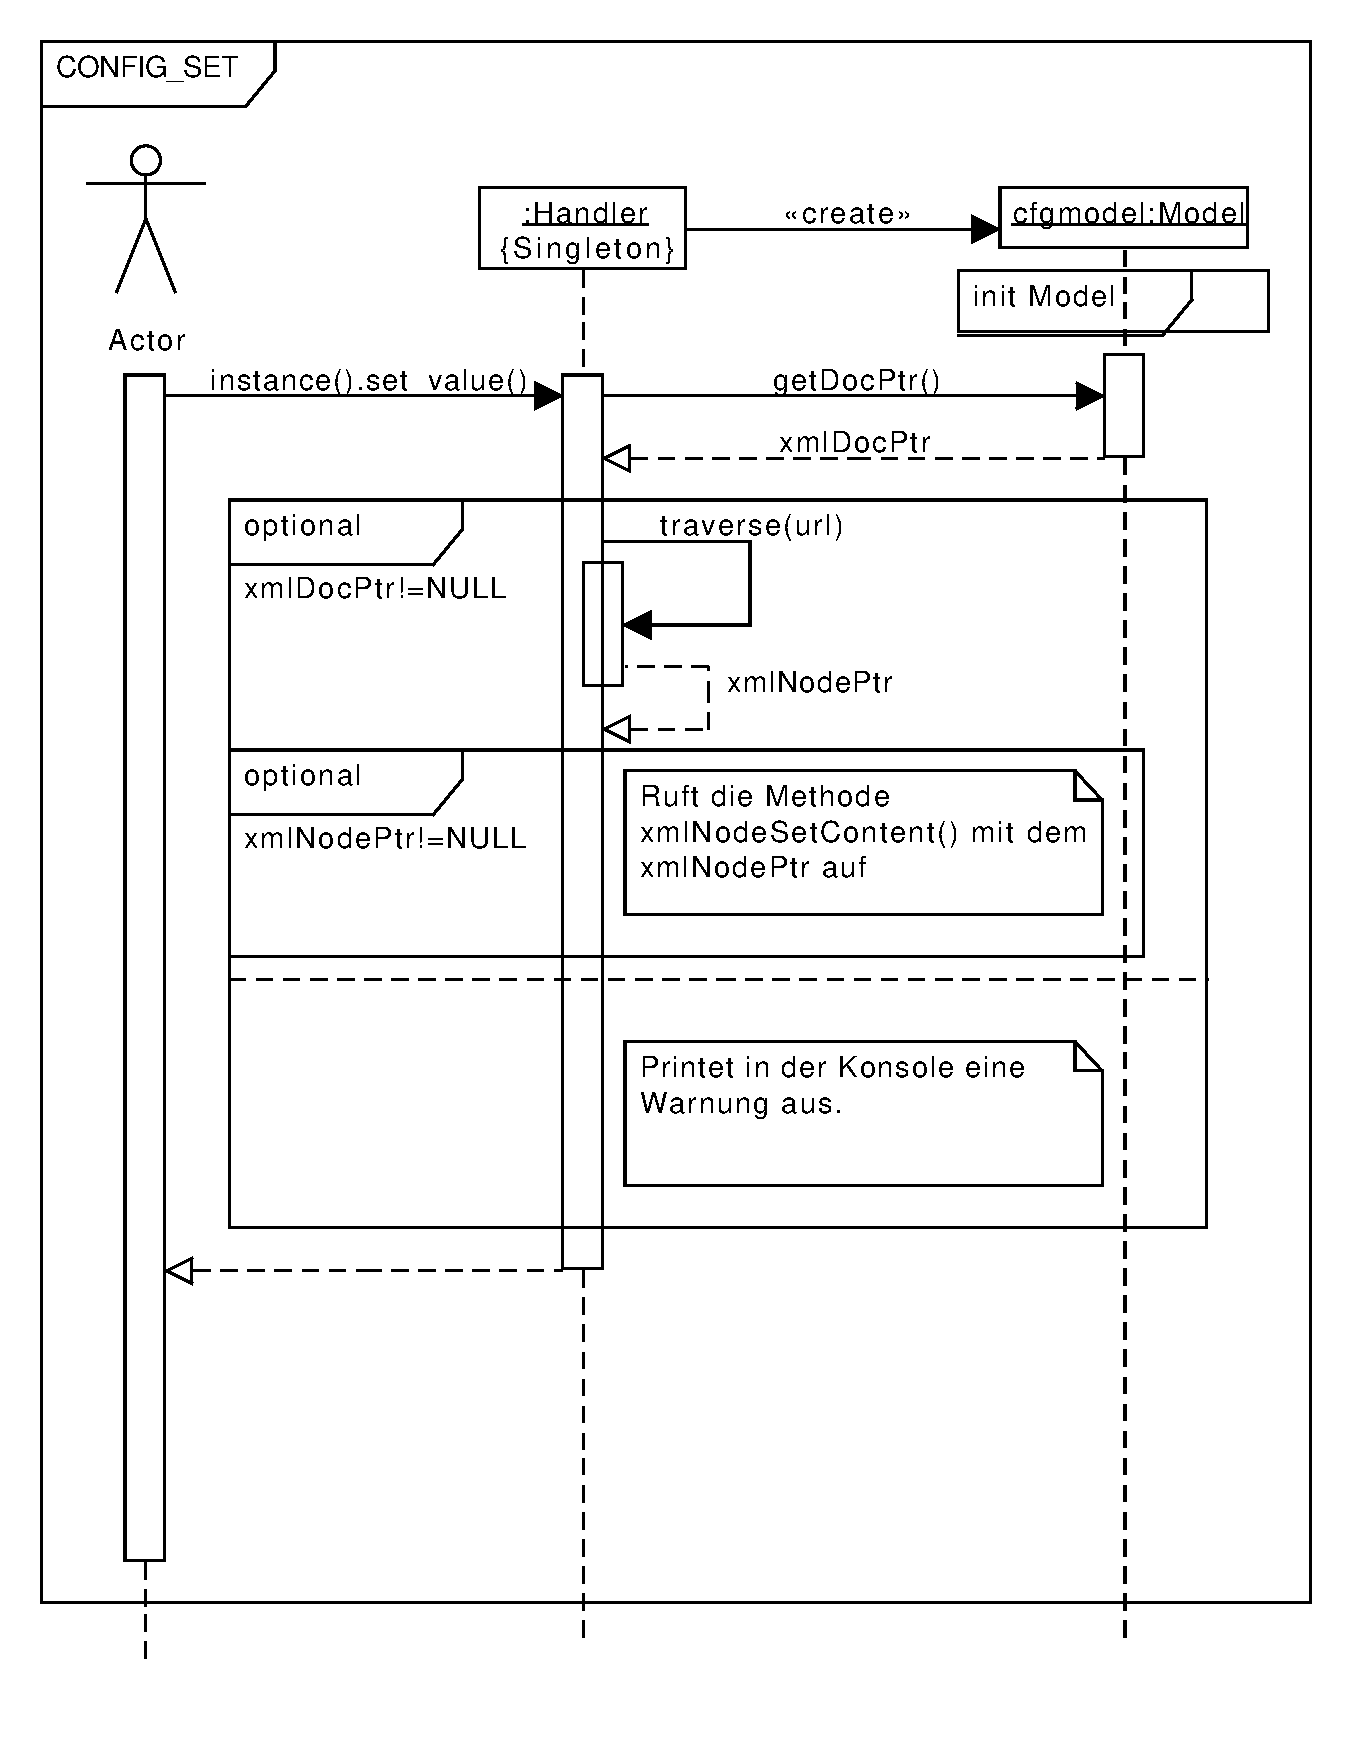
\includegraphics[scale=0.5]{configset.pdf}
%\caption{Config get\_value() Ablauf}
\label{c_configset}

Grober Ablauf beim setzen einer Integer Wertes:



\begin{itemize}

    \item Aufruf des \verb+CONFIG_SET_AS_INT("settings.connection.port",6667)+ Makros, Url ist ein ustring, Port ein Integer
    \item Über das Makro wird die Wrapper Methode \verb+set_value_as_int(Glib::ustring url,int value)+ aufgerufen
    \item Diese Methode wandelt den Integer Wert in einen String (char*) um und ruft die eigentliche set Methode 
          set\_value(url, wert) auf
    \item Die set\_value(url, wert) Methode holt sich über cfgmodel.getDocPtr(); einen aktuellen Dokument Pointer über die Model
    \item Ist der Dokument Pointer NULL, so kann kein Wert geschrieben werden, also wird über den Log:Writer
          eine entsprechende Warnung in die Logdatei geschreiben.
    \item Bei einem gültigem Dokument Pointer wird  xmlNodePtr cur = xmlDocGetRootElement(doc) aufgeruden,
          diese liefert einen xmlNodePtr (xml node pointer) auf das root Element zurück.
    \item Mittels cur->xmlChildrenNode wird der Pointer auf den folgenden Kinderknoden gesetzt und die traverse() Methode aufgerufen
     \item Nun werden diverse Vorbereitungen getätigt und anschließend rekursiv im Baum nach der übergebenen Url gesucht. Hier wird rekursiv
     der jeweilige Teilstring (teilstring1.teilstring2.teilstring2) gemäß dem Url Aufbau untersucht
           
     \item Wird die Url nicht gefunden oder sind andere Fehler aufgetreten wird ein \emph{NULL Pointer} zurückgegeben
                  und eine entsprechende Fehlermeldung in die Logdatei geschrieben
     \item Wird die die entsprechende Url gefunden, so wird der Optionswert über die Aufruferkette an die set\_value() Methode \emph{returned}.
     Hier wird dann der Wert an die entsprechende Stelle gesetzt.  
\end{itemize}




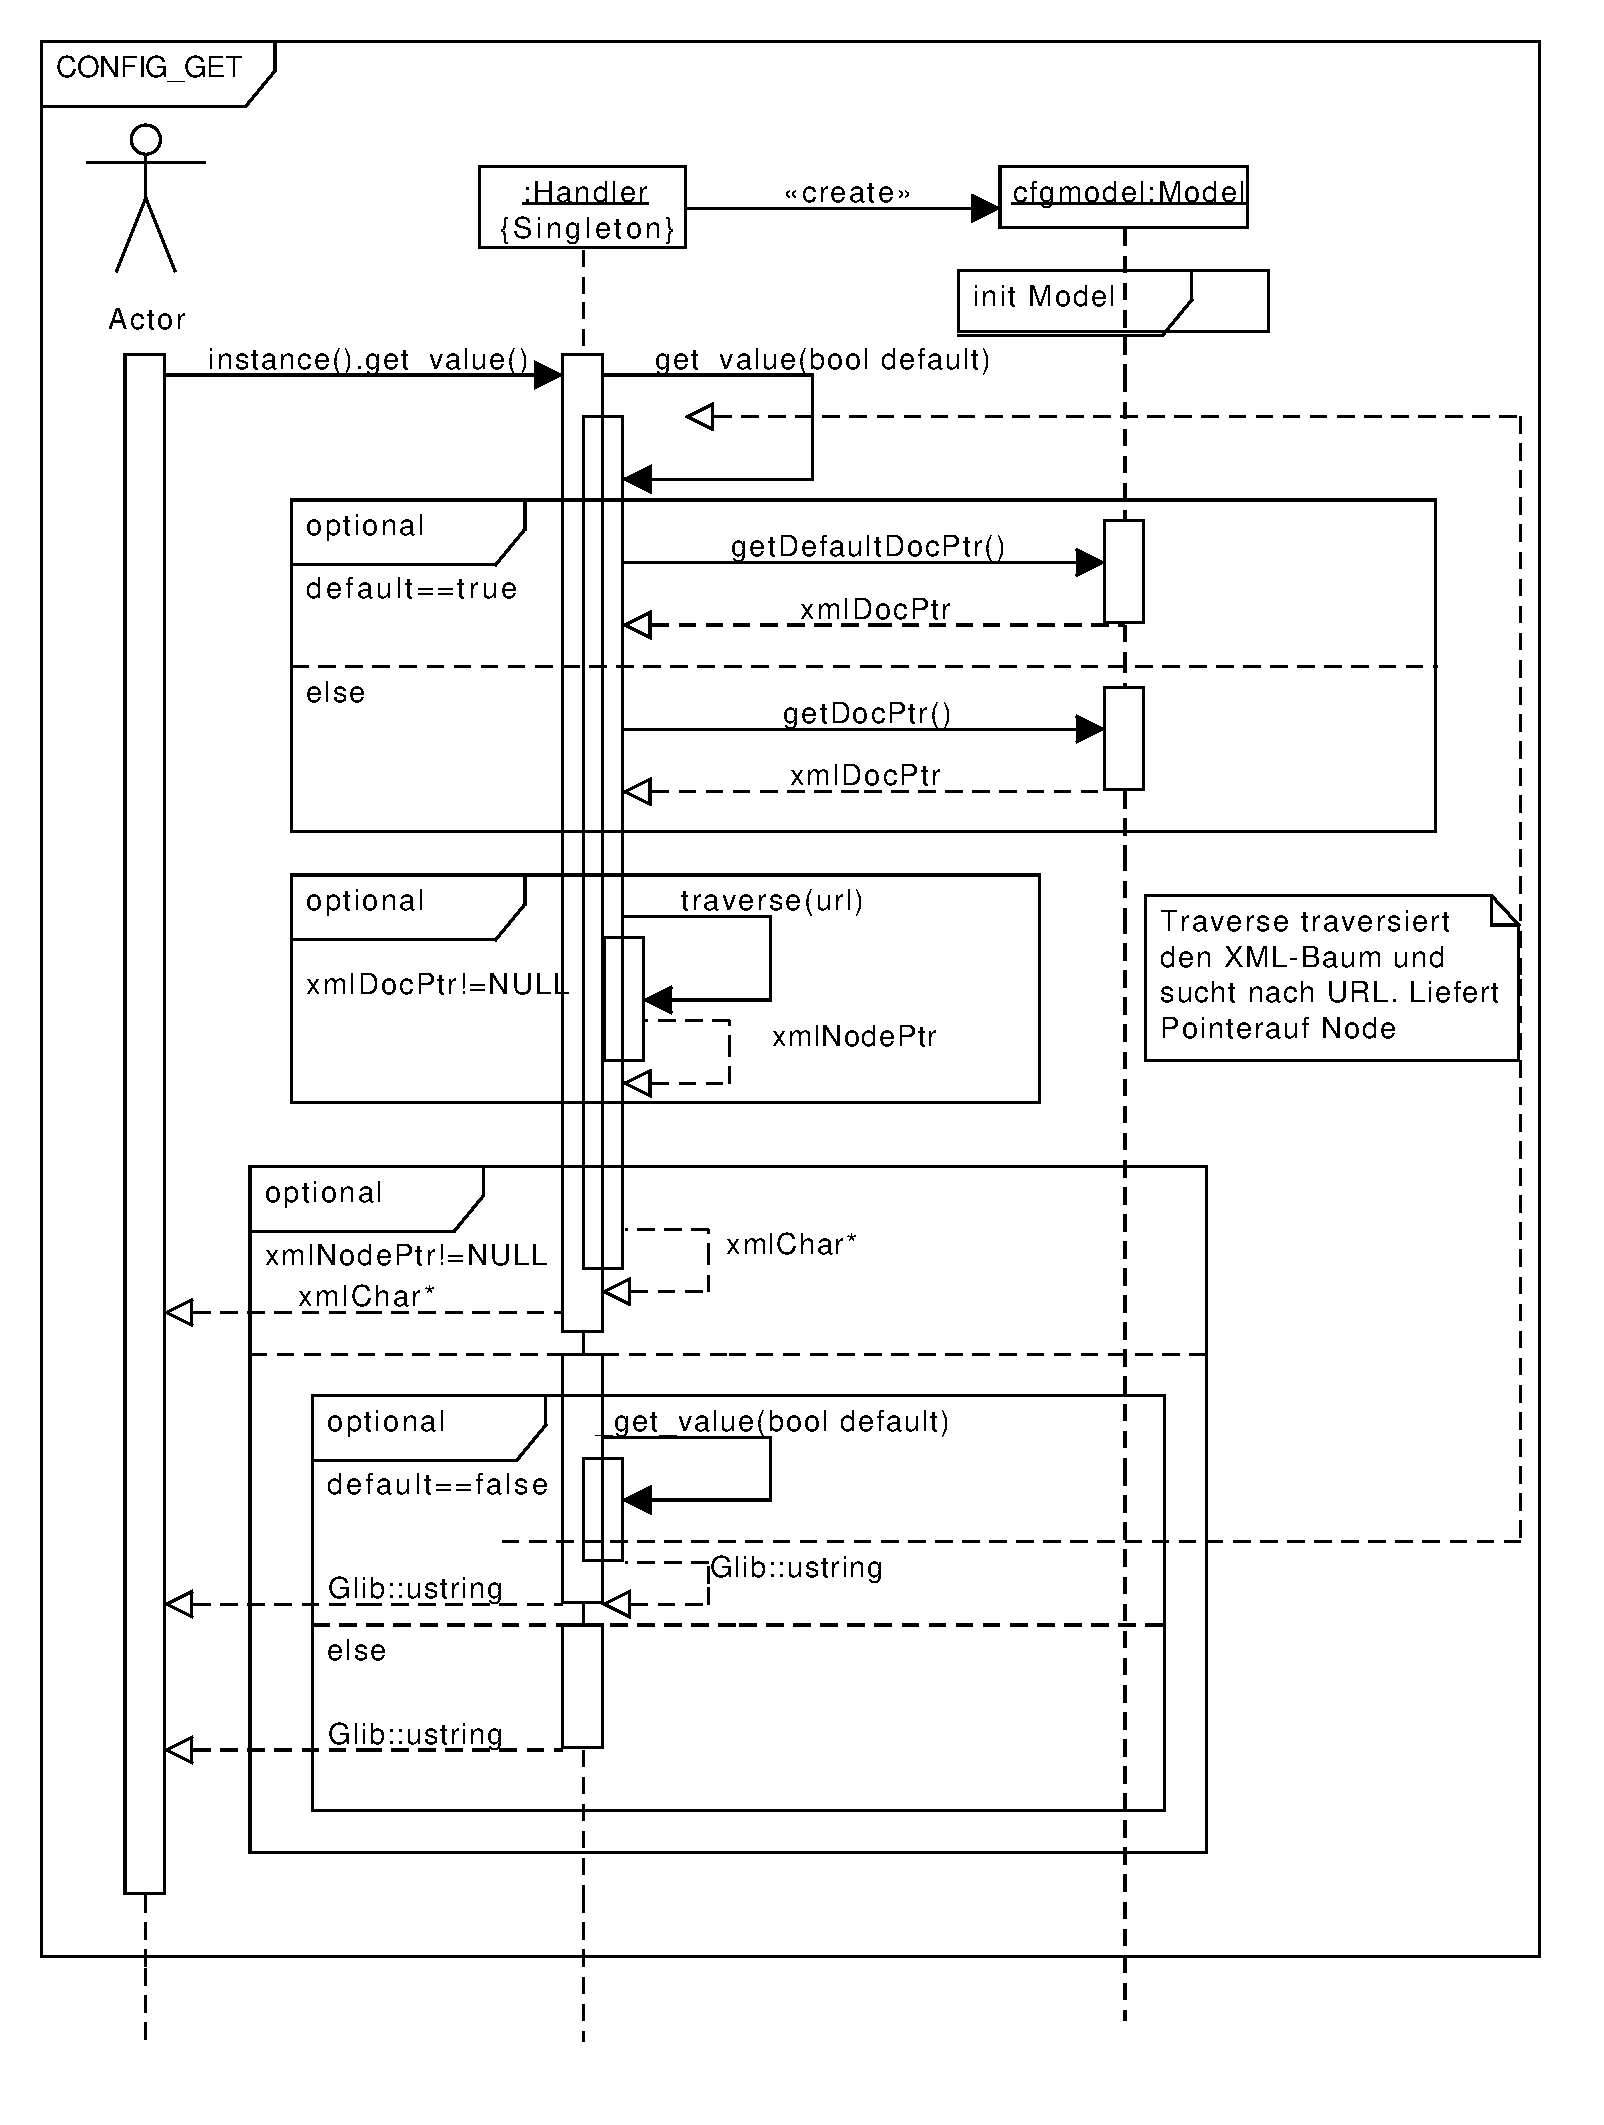
\includegraphics[scale=0.5]{configget.pdf}
%\caption{Config get\_value() Ablauf}
\label{c_configget}

%-------------------------------------------


Grober Ablauf beim Lesen eines Wertes:
\begin{itemize}


   \item Das Makro \verb+CONFIG_GET("settings.connection.host")+ wird analog dem setzen aufgerufen, dieses ruft die entsprechende Wrapper
   Methode \verb+get_value(Glib::ustring)+ welche die eigentliche \verb+_get_value(Glib::ustring url,bool getdefault)+ Methode aufruft.
   Der zweite Parameter dient dazu der \verb+_get_value()+ Methode mitzuteilen ob der entsprechende Default Wert aus der einkompilierten 
   Konfigurationsdatei oder der Custom User Wert gelanden werden soll.
   \item Die \verb+_get_value()+ Methode entsprechend dem flag, den ,,richtigen'' Dokument Pointer über das Model (analog Setzen eines Integer Wertes)
   \item Bei einen gültigen Pointer wird analog zum Setzen der Dokument Pointer auf das erste Element gesetzt und traverse
      aufgerufen (siehe Setzen eines Wertes).
   \item Kann kein Node ermittelt werden (d.h. cur Pointer zeigte auf NULL nach dem traversieren), so wird eine entsprechende Warnung über den
         Logwriter in die Logdatei geschreiben und anschließend wird die \verb+_get_value(url,true)+ Methode rekursiv mit einem true Flag aufgerufen.
         Aufgrund des true flags wird nun der Dokument Pointer mit den Default Werten über das Model geladen.
    \item Analog zum bisherigen Verlauf beim ,,Lesen eines Wertes'' erfolgt die Suche des Default Wertes. Kann am Ende kein
    Default Wert ermittelt werden so wird an den Aufrufer eine leerer ustring "" zurückgegeben.
\end{itemize}










